%%%%%%%%%%%%%%%%%%%%%%%%%%%%%%%%%%%%%%%%%
% Beamer Presentation
% LaTeX Template
% Version 1.0 (10/11/12)
%
% This template has been downloaded from:
% http://www.LaTeXTemplates.com
%
% License:
% CC BY-NC-SA 3.0 (http://creativecommons.org/licenses/by-nc-sa/3.0/)
%
%%%%%%%%%%%%%%%%%%%%%%%%%%%%%%%%%%%%%%%%%

%----------------------------------------------------------------------------------------
%	PACKAGES AND THEMES
%----------------------------------------------------------------------------------------

\documentclass{beamer}

\mode<presentation> {

% The Beamer class comes with a number of default slide themes
% which change the colors and layouts of slides. Below this is a list
% of all the themes, uncomment each in turn to see what they look like.

%\usetheme{default}
%\usetheme{AnnArbor}
%\usetheme{Antibes}
%\usetheme{Bergen}
%\usetheme{Berkeley}
%\usetheme{Berlin}
%\usetheme{Boadilla}
%\usetheme{CambridgeUS}
%\usetheme{Copenhagen}
%\usetheme{Darmstadt}
%\usetheme{Dresden}
%\usetheme{Frankfurt}
%\usetheme{Goettingen}
%\usetheme{Hannover}
%\usetheme{Ilmenau}
%\usetheme{JuanLesPins}
%\usetheme{Luebeck}
\usetheme{Madrid}
%\usetheme{Malmoe}
%\usetheme{Marburg}
%\usetheme{Montpellier}
%\usetheme{PaloAlto}
%\usetheme{Pittsburgh}
%\usetheme{Rochester}
%\usetheme{Singapore}
%\usetheme{Szeged}
%\usetheme{Warsaw}

% As well as themes, the Beamer class has a number of color themes
% for any slide theme. Uncomment each of these in turn to see how it
% changes the colors of your current slide theme.

%\usecolortheme{albatross}
%\usecolortheme{beaver}
%\usecolortheme{beetle}
%\usecolortheme{crane}
%\usecolortheme{dolphin}
%\usecolortheme{dove}
%\usecolortheme{fly}
%\usecolortheme{lily}
%\usecolortheme{orchid}
%\usecolortheme{rose}
%\usecolortheme{seagull}
%\usecolortheme{seahorse}
%\usecolortheme{whale}
%\usecolortheme{wolverine}

%\setbeamertemplate{footline} % To remove the footer line in all slides uncomment this line
%\setbeamertemplate{footline}[page number] % To replace the footer line in all slides with a simple slide count uncomment this line

%\setbeamertemplate{navigation symbols}{} % To remove the navigation symbols from the bottom of all slides uncomment this line
}

\usepackage{graphicx} % Allows including images
\usepackage{booktabs} % Allows the use of \toprule, \midrule and \bottomrule in tables

%----------------------------------------------------------------------------------------
%	TITLE PAGE
%----------------------------------------------------------------------------------------

\title[Predictions in Financial Time Series]{Predictions in Financial Time Series} % The short title appears at the bottom of every slide, the full title is only on the title page

\author{Allan Steel} % Your name
\institute[ITB] % Your institution as it will appear on the bottom of every slide, may be shorthand to save space
{
Institute of Technology Blanchardstown \\ % Your institution for the title page
\medskip
\textit{allan@allansteel.com} % Your email address
}
\date{\today} % Date, can be changed to a custom date

\begin{document}

\begin{frame}
\titlepage % Print the title page as the first slide
\end{frame}

\begin{frame}
\frametitle{Contents} % Table of contents slide, comment this block out to remove it
\tableofcontents % Throughout your presentation, if you choose to use \section{} and \subsection{} commands, these will automatically be printed on this slide as an overview of your presentation
\end{frame}

%----------------------------------------------------------------------------------------
%	PRESENTATION SLIDES
%----------------------------------------------------------------------------------------

%------------------------------------------------
\section{Introduction} %
%------------------------------------------------

%\subsection{Subsection Example} % A subsection can be created just before a set of slides with a common theme to further break down your presentation into chunks

\begin{frame}
\frametitle{Introduction}
\begin{itemize}
\item Technical Analysis
\item Time Series Analysis
\end{itemize}

\end{frame}


%------------------------------------------------
\section{Data} %
%------------------------------------------------

% ---- Frame ------------
\begin{frame}
\frametitle{Data}
\begin{itemize}
\item Financial Data - time series
\item Yahoo
\item National Indices - geographical spread
\item UK, Germany, France, US, Japan, Australia
\end{itemize}
\end{frame}

% ---- Frame ------------
\begin{frame}
\frametitle{OHLC Data}
\begin{figure}
\centering
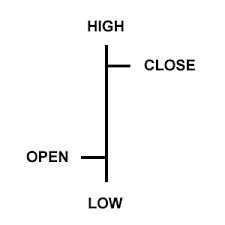
\includegraphics[width=6cm]{../Figures/chp3_ohlc}
\caption[]{A schematic representation of open, high, low and closing prices (OHLC)}
\label{fig:chp3_ohlc}
\end{figure}
\end{frame}

% ---- Frame ------------
\begin{frame}
\frametitle{German Dax}
% latex table generated in R 3.1.0 by xtable 1.7-3 package
% Wed May 28 17:41:24 2014
\begin{table}[ht]
\centering
\caption[Final 6 rows of the Dax data set.]{Final 6 rows of the Dax data set} 
\label{tab:daxtail}
\begin{tabular}{lcccc}
  \toprule Date & Open & High & Low & Close \\ 
  \midrule 13/12/2013 & 9017 & 9047 & 8991 & 9006 \\ 
  16/12/2013 & 9005 & 9188 & 8998 & 9164 \\ 
  17/12/2013 & 9143 & 9162 & 9085 & 9085 \\ 
  18/12/2013 & 9145 & 9191 & 9122 & 9182 \\ 
  19/12/2013 & 9280 & 9352 & 9257 & 9336 \\ 
  20/12/2013 & 9371 & 9413 & 9353 & 9400 \\ 
   \bottomrule \end{tabular}
\end{table}

\end{frame}

% ---- Frame ------------
\begin{frame}
\frametitle{German Dax Summary Statistics}
\begin{table}[!htbp] \centering
\caption[Dax summary statistics.]{Summary statistics of the Dax data set.}
\label{tab:daxsum}
\begin{tabular}{lccccc}
\toprule
Statistic & N & Mean & St. Dev & Min & Max \\
\midrule
Open  & 3,621 & 5,858.36 & 1,559.40 & 2,203.97 & 9,752.11 \\
High  & 3,621 & 5,906.70 & 1,561.17 & 2,319.65 & 9,794.05 \\
Low   & 3,621 & 5,804.85 & 1,557.49 & 2,188.75 & 9,714.02 \\
Close & 3,621 & 5,857.74 & 1,559.39 & 2,202.96 & 9,742.96 \\
\bottomrule
%\normalsize
\end{tabular}
\end{table}
\end{frame}

% ---- Frame ------------
\begin{frame}
\frametitle{German Dax 2000 to 2013}
\begin{figure}
\centering
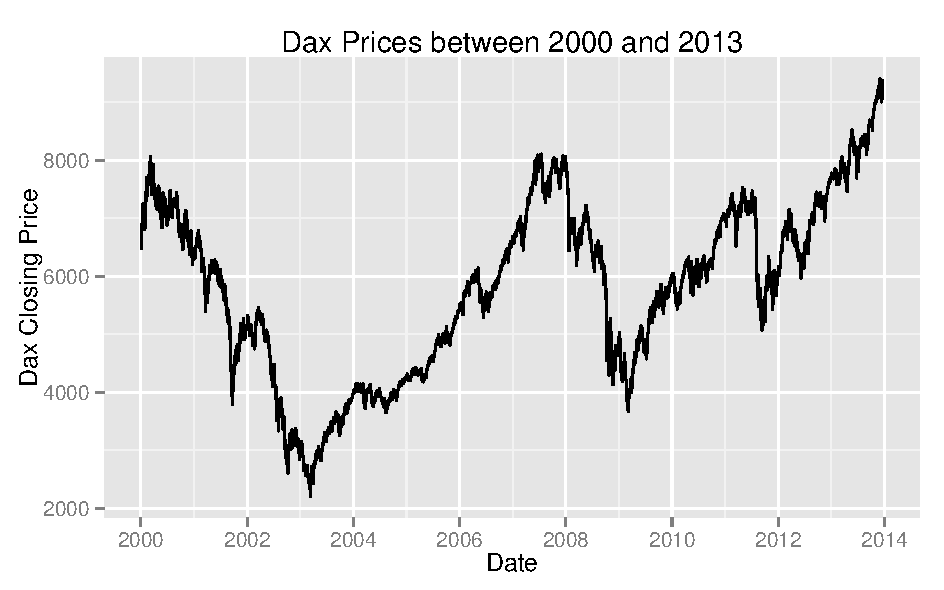
\includegraphics[width=10cm]{../Figures/chp3_dax_2000_2013}
\caption{Graph of German Dax in 2013.}
\label{fig:chp3_dax_2000_2013}
\end{figure}

\end{frame}

%------------------------------------------------
\section{Technical Analysis} %
%------------------------------------------------

% ---- Frame ------------
\begin{frame}
\frametitle{Technical Analysis}
\begin{itemize}
\item Technical analysis is the study of historical prices
\item Practitioners of technical analysis in the past were referred to as chartists
\item all that was needed to know about a particular market was contained in its pricing chart
\end{itemize}

Murphy defines technical analysis as:

\textit{\textquotedblleft Technical analysis is the study of market action, primarily through the use of charts for the purpose of forecasting future price trends.\textquotedblright}

\end{frame}

% ---- Frame ------------
\begin{frame}
\frametitle{Technical Analysis}

\textit{\textquotedblleft Obviously I am biased against the chartist. This is not only a personal predilection, but a professional one as well. Technical Analysis is anathema to the academic world. We love to pick on it. Our bullying tactics are prompted by two considerations: (1) the method is patently false; and (2) it's easy to pick on. And while it may seem a bit unfair to pick on such a sorry target, just remember: it is your money we are trying to save.\textquotedblright}

\end{frame}

%------------------------------------------------
\section{Time Series} %
%------------------------------------------------

% ---- Frame ------------
\begin{frame}
\frametitle{Time Series}

\begin{itemize}
\item ARIMA
\item Hybrid ARIMA
\end{itemize}

\end{frame}

% ---- Frame ------------
\begin{frame}
\frametitle{ARIMA}

\begin{itemize}
\item Plot the data to get a general feel for the time series and to establish if it is stationary.
\item Stabilize any variance in the data with a transformation process such as the Box-Cox method.
\item Arima models work with stationary data, so if necessary, take differences of the data until it is stationary.
\item Examine the auto-correlation and partial auto-correlation (ACF/PACF) plots in order to determine if an AR(p) or MA(q) model is appropriate.
\item Test the chosen model(s), using the AICc to determine if a better model is available.
\item Check the residuals from the best model by plotting the ACF, and doing a portmanteau test on them. If the results from these tests do not look like white noise, a modified model may be required.
\item Finally, once the residuals have a similar pattern to white noise, the model can be used to generate forecasts.
\end{itemize}

\end{frame}

%------------------------------------------------
\section{Results} %
%------------------------------------------------

\begin{frame}

\frametitle{Results}
\begin{itemize}
\item Introduction
\item Data
\end{itemize}

\end{frame}


%------------------------------------------------

\begin{frame}
\Huge{\centerline{The End}}
\end{frame}

%----------------------------------------------------------------------------------------

\end{document} 